\documentclass[11pt,a4paper]{article}
\usepackage[spanish,es-nodecimaldot]{babel}	% Utilizar español
\usepackage[utf8]{inputenc}					% Caracteres UTF-8
\usepackage{graphicx}						% Imagenes

\PassOptionsToPackage{hyphens}{url}
\usepackage[hidelinks]{hyperref}			% Poner enlaces sin marcarlos en rojo

\usepackage{fancyhdr}						% Modificar encabezados y pies de pagina
\usepackage{float}							% Insertar figuras
\usepackage[textwidth=390pt]{geometry}		% Anchura de la pagina
\usepackage[nottoc]{tocbibind}				% Referencias (no incluir num pagina indice en Indice)
\usepackage{enumitem}						% Permitir enumerate con distintos simbolos
\usepackage[T1]{fontenc}					% Usar textsc en sections
\usepackage{amsmath}						% Símbolos matemáticos
\usepackage{listings}
\usepackage{algorithm}
\usepackage{amssymb}

\usepackage[
backend=biber,
style=numeric,
sorting=ynt
]{biblatex}
 
\addbibresource{mybib.bib}

% no accents in math operators
\unaccentedoperators

\usepackage{color}
 
\definecolor{codegreen}{rgb}{0,0.6,0}
\definecolor{codegray}{rgb}{0.5,0.5,0.5}
\definecolor{codepurple}{rgb}{0.58,0,0.82}
\definecolor{backcolour}{rgb}{0.95,0.95,0.92}
 
\lstdefinestyle{mystyle}{
    backgroundcolor=\color{backcolour},   
    commentstyle=\color{codegreen},
    keywordstyle=\color{magenta},
    numberstyle=\tiny\color{codegray},
    stringstyle=\color{codepurple},
    basicstyle=\footnotesize,
    breakatwhitespace=false,         
    breaklines=true,                 
    captionpos=b,                    
    keepspaces=true,                 
    numbers=left,                    
    numbersep=5pt,                  
    showspaces=false,                
    showstringspaces=false,
    showtabs=false,                  
    tabsize=2
}
 
\lstset{style=mystyle, language=Python}

% Comando para poner el nombre de la asignatura
\newcommand{\asignatura}{Visión por Computador}
\newcommand{\autor}{Vladislav Nikolov Vasilev}

% Configuracion de encabezados y pies de pagina
\pagestyle{fancy}
\lhead{Vladislav Nikolov, José María Sánchez}
\rhead{\asignatura{}}
\lfoot{Grado en Ingeniería Informática}
\cfoot{}
\rfoot{\thepage}
\renewcommand{\headrulewidth}{0.4pt}		% Linea cabeza de pagina
\renewcommand{\footrulewidth}{0.4pt}		% Linea pie de pagina

\begin{document}
\pagenumbering{gobble}

% Pagina de titulo
\begin{titlepage}

\begin{minipage}{\textwidth}

\centering

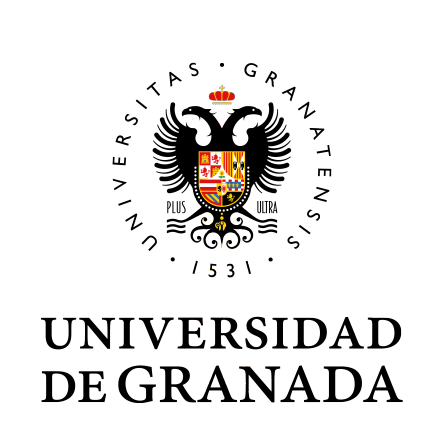
\includegraphics[scale=0.5]{img/ugr.png}\\

\textsc{\Large \asignatura{}\\[0.2cm]}
\textsc{GRADO EN INGENIERÍA INFORMÁTICA}\\[1cm]

\noindent\rule[-1ex]{\textwidth}{1pt}\\[1.5ex]
\textsc{{\Huge PROYECTO FINAL\\[0.5ex]}}
\noindent\rule[-1ex]{\textwidth}{2pt}\\[3.5ex]

\end{minipage}

\vspace{1cm}

\begin{minipage}{\textwidth}

\centering

\textbf{Autores}\\ {\autor{}}\\{José María Sánchez Guerrero}\\[2ex]
\textbf{Rama}\\ {Computación y Sistemas Inteligentes}\\[2ex]
\vspace{0.3cm}


\includegraphics[scale=0.3]{img/etsiit.jpeg}

\vspace{0.7cm}
\textsc{Escuela Técnica Superior de Ingenierías Informática y de Telecomunicación}\\
\vspace{1cm}
\textsc{Curso 2018-2019}
\end{minipage}
\end{titlepage}

\pagenumbering{arabic}
\tableofcontents
\thispagestyle{empty}				% No usar estilo en la pagina de indice


\newpage

\setlength{\parskip}{1em}

\section{\textsc{Descripción del problema}}

El problema que hemos escogido al alimón consiste en adaptar una red siamesa a un nuevo problema.
En este caso, vamos a adaptar una red preentrenada con imágenes de caras al problema de determinar
si dos personas están emparentadas o no a partir de fotos de sus caras. Este es un problema perfecto
para un tipo de red así, ya que normalmente redes de este tipo se utilizan en problemas de reconocimiento
facial (por ejemplo, determinar si dos fotos pertenecen o no a la misma persona). Por tanto, coger una red
de este tipo y aplicarla a un problema en el que también tenemos que comparar caras de personas
para determinar si están emparentadas parece lógico.

El conjunto de datos con el que vamos a trabajar es el \textbf{\textit{Recognizing Faces in the Wild}} \cite{faces},
creado por SMILE Lab de la Universidad de Northeastern, y contiene una serie de directorios los cuales
pertenecen a distintas familias. Cada una de estas familias está formada por uno o más individuos,
de los que se dispone de una o más fotos.

El conjunto de datos viene dividido en \textit{training} y test. El conjunto de entrenamiento sigue la estructura
anteriormente definida y viene acompañado de un archivo llamado ``\textit{train\_relationships.csv}'', el
cuál indica las relaciones de parentesco entre los individuos de las distintas familias (solo las relaciones
positivas, unas 3598). No obstante, el conjunto de test no sigue la estructura de directorios anteriormente descrita,
si no que vienen las imágenes sueltas acompañadas del archivo ``\textit{sample\_submission.csv}'', el cuál
indica las parejas de imágenes que se quiere verificar si son o no parientes.

En el conjunto de entrenamiento disponemos de unas 786 familias. En total tenemos unos 3965 individuos, y cada
familia está compuesta por un número variable de estos. Las imágenes que tenemos están a color y tienen un
tamaño de $224 \times 224$ píxeles. En total disponemos de 20726 imágenes de entrenamiento. No obstante, sería
interesante dejar una parte de las imágenes para validar el modelo, para ver cómo lo va haciendo con datos
que nunca antes a visto a medida que va entrenando. En secciones posteriores explicaremos cómo
hemos determinado con qué imágenes entrenar y cuántas imágenes serán de validación y cómo se irán generando.

El conjunto de test está formado por 4866 imágenes de las mismas características que las de entrenamiento.
Además, como hemos dicho anteriormente, disponemos de un archivo en formato \texttt{CSV} que indica
las parejas de imágenes para las que se quiere determinar si son parientes o no. Ya que disponemos de este
conjunto de datos, vamos a utilizarlo para ver cómo de bien lo hace nuestro modelo con imágenes nunca antes
vistas. Como no disponemos de las etiquetas reales, la forma de comprobar los resultados será rellenar el archivo
\texttt{CSV} anterior con las predicciones y subirlo a \textit{Kaggle}, donde en unos pocos segundos obtendremos
la \textit{accuracy} que hemos obtenido.

En cuanto a la salida, debido a la naturaleza del problema, la red va a obtener un valor entre 0 y 1.
El valor 0 representa que las dos personas no están emparentadas, mientras que el 1 representa que
están emparentadas. Los valores intermedios dirán que hay un determinado grado de parentesco entre
las dos personas. Como no disponemos de un valor umbral para determinar a partir del que podamos discernir
si dos personas están emparentadas o no, subiremos los resultados a \textit{Kaggle} y veremos cómo de buenos
han sido.

Es muy importante destacar, antes de continuar, que estamos ante un problema muy difícil y terriblemente
desbalanceado, ya que el número de relaciones de parentesco de las que disponemos es muchísimo menor frente
al número de relaciones de no parentesco que existen.

\section{\textsc{Enfoque elegido}}

A continuación vamos a presentar el enfoque que hemos elegido para desarrollar el proyecto. Los pasos
que vamos a seguir son los siguientes:

\begin{enumerate}
    \item Lo primero que vamos a hacer es dividir los datos de entrenamiento de los que disponemos
    en dos conjuntos: uno de entrenamiento, donde tendremos los datos con los que podremos entrenar
    la red, y un conjunto de validación, con el que podremos validar el modelo a medida que lo vamos entrenando.
    \item Vamos a crear generadores de datos para entrenar y validar el modelo. El motivo de esto será explicado
    más adelante.
    \item Vamos a partir de una serie de modelos base preentrenados y vamos a comprarlos para ver cómo se comportan.
    Una vez que tengamos los resultados, elegiremos el mejor de ellos.
    \item Una vez que hemos elegido el mejor modelo base, vamos a hacerle un ajuste fino con el objetivo
    de mejorar los resultados obtenidos. Compararemos los resultados que obtenemos con cada mejora y nos quedaremos
    con la que funcione mejor.
    \item Finalmente, valoraremos los resultados obtenidos y extraeremos conclusiones.
\end{enumerate}

Antes de continuar, vamos a hablar brevemente de las redes que vamos a utilizar.

\section{\textsc{Redes a utilizar}}

Para evitar tener que crear las redes y entrenarlas de cero, vamos a partir, tal y como hemos dicho anteriormente,
de una serie de redes preentrenadas. Dichas redes han sido entrenadas con el conjunto de datos \texttt{VGGFace2},
creado por la Universidad de Oxford \cite{vggface2}, el cuál contiene más de 3.3 millones de caras.

Las implementaciones oficiales de las redes están hechas en \texttt{Pytorch}. Sin embargo, nosotros vamos a utilizar
\texttt{Keras}. Por tanto, hemos buscado alguna implementación que estuviese hecha en el \textit{framework}
que vamos a utilizar, y hemos dado con un proyecto en GitHub \cite{keras-vggface}. Dicho proyecto
dispone de tres redes ya entrenadas con \texttt{VGGFace2}: \texttt{VGG16}, \texttt{ResNet-50} y \texttt{SeNet-50}.
Además, las redes tienen su función de preprocesamiento, con lo cuál nos podemos olvidar de hacerlo nosotros
mismos. Vamos a partir de estas tres redes básicas y veremos cuál es la que funciona mejor de ellas. Sobre
aquella que consideremos mejor, aplicaremos posteriormente mejoras para ver hasta dónde podemos mejorar
nuestro modelo.

Es importante destacar que las redes como tales no son siamesas. Por tanto, tendremos que modificar ligeramente
las redes ya entrenadas para que funcionen como redes siamesas. Estas modificaciones se explicarán posteriormente.

\section{\textsc{Lectura y procesamiento de datos}}

En esta sección vamos a ver cómo leemos los datos de entrada y como los preprocesamos para poder trabajar con
ellos de una forma más cómoda. Lo primero que haremos será pasar la ruta donde tenemos guardado nuestro
\textit{dataset} a una función, y a partir de ella, obtendremos una lista con todos los miembros de cada familia
y un diccionario con las rutas de las imágenes disponibles de cada individuo. La función que nos permite esto
es la siguiente:

\begin{lstlisting}
def read_family_members_images(data_path):
    """
    Funcion que procesa la ruta especificada como parametro. Obtiene
    una lista con los miembros de cada familia, la cual tendra el
    formato "FXXXX/MIDY", y un diccionario con las rutas de las
    imagenes de cada miembro de cada familia.

    Args:
        data_path: Ruta de los archivos a procesar.
    
    Return:
        Devuelve una lista con los miembros de cada familia y un
        diccionario con las imagenes de cada miembro de cada familia.
    """
    # Leer la ruta proporcionada y obtener todos los directorios
    # Cada directorio esta asociado a una familia
    dirs = sorted(list(glob.glob(data_path + "*")))

    # Obtener los nombres de los directorios de las familias
    family_dirs = np.array([dir.split("/")[-1] for dir in dirs])

    # Obtener imagenes asociadas a cada directorio
    images = {f"{family}/{member.split('/')[-1]}": sorted(list(glob.glob(member + "/*.jpg")))
        for family in family_dirs for member in sorted(list(glob.glob(f"{data_path}{family}/*")))
    }
    
    family_members_list = list(images.keys())
    
    return family_members_list, images
\end{lstlisting}

Una vez disponemos de las rutas de las imágenes, ahora tendremos que leerlas. Para ello utilizamos una función a
la cual le pasamos una de las rutas obtenidas y nos cargará la imagen como un array de números reales.
Posteriormente, preprocesamos la imagen gracias a la función de preprocesado proporcionada por el módulo
del que hemos hablado anteriormente. Dicha función de lectura de imágenes se puede ver a continuación:

\begin{lstlisting}
def read_image(path):
    """
    Funcion que permite leer imagenes a partir de un archivo
    Args:
        path: Ruta de la imagen
    """
    img = cv2.imread(path)
    img = np.array(img).astype(np.float)
    return preprocess_input(img, version=2)
\end{lstlisting}

Podemos ver en la función de preprocesado que tenemos un parámetro \texttt{version}. Este parámetro habrá que
establecerlo, como nos dice el propio autor, en 1 para \texttt{VGG16} o en 2 para \texttt{ResNet-50} y
\texttt{SeNet-50}.

\section{\textsc{División y generación de datos}}

Una vez que hemos leído los datos y hemos generado la lista de individuos y el diccionario
que permite acceder a las imágenes de cada individuo, vamos a dividir la lista de individuos
que tenemos en dos conjuntos, uno de entrenamiento y uno de validación. Hemos decidido hacer
la división por individuos porque es la que parece más natural, ya que queremos comparar una
imagen de un individuo con una imagen de otro, independientemente de si son de la misma familia
o no, ya que en el mundo real puede que no tengamos disponible esa información.

Dividir por imágenes no tiene mucho sentido, ya que podríamos tener imágenes de un mismo individuo
en los dos conjuntos, y eso no es lo que buscamos. Nos interesa que los datos de validación sean
completamente nuevos. Tampoco consideramos que sea buena idea dividir por familias porque entonces
estamos restringiendo demasiado las posibles combinaciones. A lo mejor las familias que se dejan
fuera son demasiado difíciles para que la red pueda acertarlas correctamente.

Hemos establecido que el 80\% de los individuos totales estén en el conjunto de entrenamiento, mientras
que solo el 20\% esté en el de validación. Hemos considerado que estos porcentajes son los adecuados,
ya que no se pierden demasiados datos de entrenamiento y el conjunto de validación no es demasiado
pequeño.

Para hacer la división hemos utilizado la siguiente función:

\begin{lstlisting}
def generate_datasets(families, val_prop=0.2):
    """
    Funcion que permite generar los datasets de train, test y
    validacion a partir de un array de directorios, los cuales
    representan las familias. Los datos son mezclados para que
    se escoja de forma aleatoria.

    Args:
        families: Array con los directorios de las familias.
        test_prop: Proporcion de los datos totales que tiene
                   que estar en el conjunto de test.
        val_prop: Proporcion de los (datos_totales - datos_test)
                  que tienen que estar en el conjunto de validacion.
    
    Return:
        Devuelve un array con los directorios de las familias que
        forman el conjunto de train, otro para el conjunto de
        validacion y otro para el conjunto de test.
    """
    # Mezclar familias
    shuffle_families = np.copy(families)
    np.random.shuffle(shuffle_families)

    # Obtener la ultima proporcion de las familias y guardarla en
    # el conjunto de validacion
    idx_val = int(len(shuffle_families) * (1 - val_prop))
    val_dirs = shuffle_families[idx_val:]
    train_dirs = shuffle_families[:idx_val]

    # Volver a mezclar familias del conjunto de entrenamiento
    np.random.shuffle(train_dirs)

    return train_dirs, val_dirs
\end{lstlisting}

Debido a que el número de parejas de imágenes que se pueden formar es del orden de millones
y a que tenemos restricciones muy fuertes sobre el \textit{hardware} y el tiempo de los que disponemos,
no nos podemos permitir entrenar y validar el modelo con cada posible pareja. Para solventar esto, podemos
crear nuestros propios generadores de datos, de manera que controlemos en todo momento como se están generando
los \textit{batches} de entrenamiento y de validación.

Un \textit{batch} estará compuesto por $N$ parejas de imágenes (como estamos trabajando con una red siamesa, esta
va a tener dos o más entradas, aunque en nuestro caso serán dos). Tenemos que rellenar el \textit{batch} tanto con
ejemplos positivos como con negativos, controlando la proporción de ejemplos positivos que hay, ya que hay
muchos menos que ejemplos negativos. Primero introduciremos ejemplos positivos extraídos del \texttt{CSV}, comprobando
si cada uno de los individuos de la pareja están en el conjunto de entrenamiento. Una vez que hemos generado los
ejemplos positivos, creamos los negativos, escogiendo parejas aleatorias del conjunto de entrenamiento y comprobando
que no están en el archivo de relaciones positivas. Finalmente, mezclamos las parejas junto con sus etiquetas
de forma que los ejemplos positivos y los negativos estén intercalados.

Para hacer esto, podemos utilizar la siguiente función:

\begin{lstlisting}
def dataset_to_images(dataset, images, relationships, size, 
                      elationships_prop):
    """
    Funcion que genera dos arrays de individuos con un tamanio determinado, y otro que
    nos indica el parentesco entre un par de individuos de cada uno de los arrays anteriores.
    Los datos se escogeran de forma aleatoria entre todos los individuos proporcionados.
    Args:
        dataset: Array con los directorios de las familias.
        images: Array con los directorios de las imagenes de cada individuo de la familia.
        relationships: Relaciones entre los individuos a procesar.
        size: Tamanio de los datos a generar.
        relationships_prop: Proporcion de individuos con un parentesco familiar que tendran
                            los datos generados.
    
    Return:
        Devuelve dos arrays con los individuos que seran procesados por cada una de las
        partes de nuestra red, y un array con los parentescos entre los arrays anteriores
    """    
    left_images = []
    right_images = []
    targets = []

    # Elegir los 1's
    while len(left_images) < int(size*relationships_prop):
        # Escogemos una linea aleatoria del CSV
        index = np.random.choice(len(relationships))
        ind = relationships[index]

        # Comprobamos que los individuos estan en el dataset
        if ind[0] in dataset and ind[1] in dataset:
            # Elegimos aleatoriamente una imagen de esos individuos
            left_images.append(read_image(np.random.choice( images[ind[0]] )))
            right_images.append(read_image(np.random.choice( images[ind[1]] )))
            targets.append(1.)

    # Elegir los 0's
    while len(left_images) < int(size):
        # Accedemos dos individuos diferentes aleatorios del dataset
        ind = np.random.choice(dataset, 2, replace=False)

        # Comprobamos si son parientes
        if (ind[0],ind[1]) not in relationships and (ind[1],ind[0]) not in relationships:
            # En caso afirmativo aniadimos con etiqueta 1
            left_images.append( read_image( np.random.choice(images[ind[0]]) ) )
            right_images.append( read_image( np.random.choice(images[ind[1]]) ) )
            targets.append(0.0)
    
    left_images = np.array(left_images)
    right_images = np.array(right_images)
    targets = np.array(targets)

    idx_perm = np.random.permutation(size)

    left_images = left_images[idx_perm]
    right_images = right_images[idx_perm]
    targets = targets[idx_perm]

    return left_images, right_images, targets
\end{lstlisting}


Esta función devuelve un único \textit{batch}. Si queremos generar datos continuamente, podemos hacerlo
de la siguiente forma:

\begin{lstlisting}
def batch_generator(dataset, images, relationships_path,
                    batch_size=32, relationships_prop=0.2):
    """
    Funcion que selecciona aleatoriamente dos conjunto de individuos
    y sus etiquetas, asigna una proporcion de parejas con parentesco
    entre los dos conjuntos, y devuelve en cada iteracion la
    cantidad asignada como tamanio de batch.
    Args:
        dataset: Array con los directorios de las familias.
        images: Array con los directorios de las imagenes de cada
                individuo de la familia.
        relationships_path: Ruta del archivo de relaciones a procesar.
        batch_size: Tamanio del batch.
        relationships_prop: Proporcion de individuos con un parentesco
                            familiar tendran los datos generados.
    
    Return:
        Devuelve dos arrays con los individuos que seran procesados
        por cada una de las partes de nuestra red, y un array con los
        parentescos entre los arrays anteriores
    """
    # Leemos el archivo donde se encuentran las relaciones familiares
    # entre individuos
    relationships = pd.read_csv(relationships_path)
    relationships = list(zip(relationships.p1.values,
                             relationships.p2.values))
    
    while True:
        # Generamos un conjunto de imagenes aleatorias y lo devolvemos
        # hasta que el iterador vuelva a pedir otro
        left_images, right_images, targets = dataset_to_images(dataset, images, relationships, batch_size, relationships_prop)

        yield [left_images, right_images], targets
\end{lstlisting}


\section{\textsc{Generación de datos de salida}}

A la hora de generar la salida a partir del conjunto de test, hemos utilizado la funcionalidad que se implementa
en uno de los proyectos asociados al problema \cite{project}. Gracias a ella, leemos todas las parejas de imágenes de
nuestro archivo '\textit{sample\_submission.csv}' y se las pasamos a la red siamesa. Una vez obtenidos
los valores, se genera otro archivo con la misma estructura que el anterior, pero con los nuevos resultados.

\section{\textsc{Diseño y elección de la red base}}

En esta sección vamos a tratar el diseño de las redes siamesas base y la elección de la mejor de ellas.
También explicaremos cómo hemos entrenado las redes, justificando el por qué de cada decisión que hemos
tomado.

\subsection{Diseño de la arquitectura de las redes siamesas base}

Vamos a comenzar hablando sobre la arquitectura de cada red. Recordemos que vamos a probar tres redes
preentrenadas en el conjunto de datos \texttt{VGFace2}: \texttt{VGG16}, \texttt{ResNet-50} y \texttt{SeNet-50}.
Estas redes por sí mismas no son redes siamesas, pero podemos utilizarlas para extraer características gracias
a lo que ya han aprendido, adaptando claro está dicho conocimiento al problema concreto. Con algunas pequeñas
modificaciones, podemos montar una red siamesa utilizando estas redes.

Para tener más claro como son este tipo de redes, vamos a ver un ejemplo de la arquitectura de una red
siamesa:

\begin{figure}[H]
    \centering
    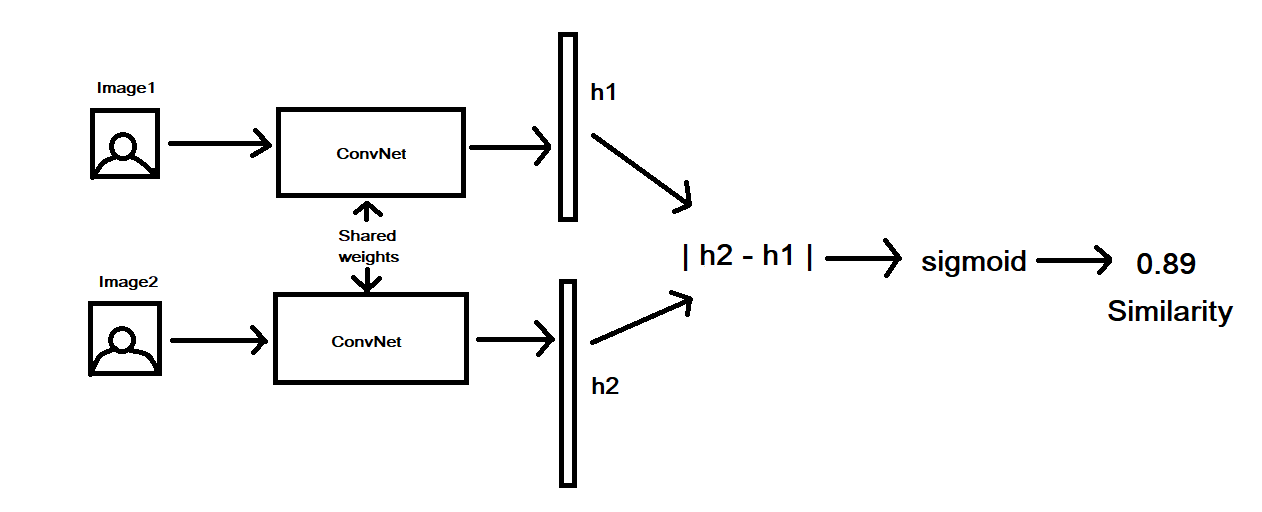
\includegraphics[scale=0.3]{img/siamese-net-arch.png}
    \caption{Ejemplo de arquitectura de una red siamesa.}
    \label{fig:siamese-net-arch}
\end{figure}

En general tenemos dos o más redes convolucionales que son idénticas (dependiendo del número de imágenes de
entrada que tengamos), ya que comparten tanto pesos como estructura. Las redes funcionan como \textit{encoders},
ya que a cada una de ellas se le pasa una imagen y obtienen un tensor de salida con las características de la imagen.
Con dichas características extraídas se aplica alguna medida de distancia, como podría
ser la distancia \textit{L1}, la \textit{L2} o cualquier otra. Finalmente, podemos tener una pequeña red
de capas densas, acabando en una capa que utiliza como función de activación la función sigmoide, la cuál
da una medida del grado de similitud entre las dos imágenes (0 significa que no tienen ningún tipo de similitud
y 1 significa que son iguales). Esto nos puede recordar a lo que explicamos al principio, donde medimos
si dos individuos están emparentados con un valor real entre 0 y 1.

En nuestro caso, vamos a tener dos redes que comparten pesos. Cada una de ellas recibirá como entrada
una imagen y extraerá características de ellas. Sobre estas características se pondrá una capa de
\texttt{GlobalMaxPooling2D}, de forma que tengamos un tensor más simple al final del proceso. Hemos escogido
este tipo de \textit{pooling} ya que nos permite quedarnos con la información más relevante. Una vez que tengamos
los dos tensores de salida, se calculará la distancia \textit{L1} entre ellos. Hemos decidido utilizar esta medida
de distancia ya que es fácil y rápida de calcular. Además, tras hacer algunas pruebas, parece que es la que mejor
funciona, ya que otras distancias como la \textit{L2} o la \textit{cosine similarity} hacen que la red siamesa se
quede estancada en el entrenamiento. Finalmente, pondremos una capa densa con función de activación sigmoide,
de forma que obtendremos un valor real entre 0 y 1 que indique el grado de similitud.

Para crear las redes, podemos utilizar la siguiente función:

\begin{lstlisting}[caption={Función para crear los modelos base.}, label={lst:base-net}]
def create_siemesenet(model, optimizer, loss_function):
    """
    Funcion que crea una red siamesa a partir de una serie de redes preentrenada
    con el conjunto de datos VGGFace2. Este modelo declara dos entradas y,
    posteriormente se conectan cada una de las partes mediante la distancia L1.
    
    Args:
        model: Indica cual de las tres redes ya entrenadas con VGGFace2
               utilizaremos en nuestro modelo: VGG16, ResNet-50 o SeNet-50
        optimizer: Indica cual sera el optimizador de nuestro modelo. Se puede
                   crear una instancia antes de pasarlo, o puede llamarlo
                   directamente por su nombre.
        loss_function: Indica la funcion de perdida de nuestro modelo. Se puede
                       pasar el nombre de una funcion de perdida existente o
                       pasar una funcion simbolica.
    
    Return:
        Devuelve la red ya creada y muestra un resumen de esta
    """
    # Dimension de los datos de entrada
    shape = (224, 224, 3)

    # Declaramos 2 entradas, una para cada imagen
    left_input = Input(shape)
    right_input = Input(shape)

    # Generamos nuestro modelo entrenado con VGGFace
    vgg_model = VGGFace(model=model, include_top=False, weights="vggface", pooling="max")

    # Codificamos las entradas utilizando la red anterior
    encoded_l = vgg_model(left_input)
    encoded_r = vgg_model(right_input)

    # Obtenemos la distancia L1 entre los dos tensores
    L1_layer = Lambda(lambda tensor:K.abs(tensor[0] - tensor[1]))

    # Aniadimos la funcion de distancia y la ultima capa sigmoidal a la red
    L1_distance = L1_layer([encoded_l, encoded_r])
    prediction = Dense(1, activation='sigmoid')(L1_distance)

    # Creamos el modelo
    siamese_net = Model(inputs=[left_input, right_input], outputs=prediction)
    # Compilamos con un optimizador y una funcion de perdida determinadas
    siamese_net.compile(loss=loss_function, optimizer=optimizer, metrics=['accuracy'])
    # Mostramos un resumen de la red
    siamese_net.summary()

    return siamese_net
\end{lstlisting}

Para crear la función anterior nos hemos basado en un proyecto de \textit{Kaggle} \cite{hulk}, modificando algunas
partes, como por ejemplo el tipo de \textit{pooling} utilizado, para adaptarla a lo anteriormente explicado.
Posteriormente, modificaremos la función de creación de la red, pero eso se verá en secciones posteriores.

Con la función anterior hemos creado las siguientes redes siamesas:

\begin{figure}[H]
    \centering
    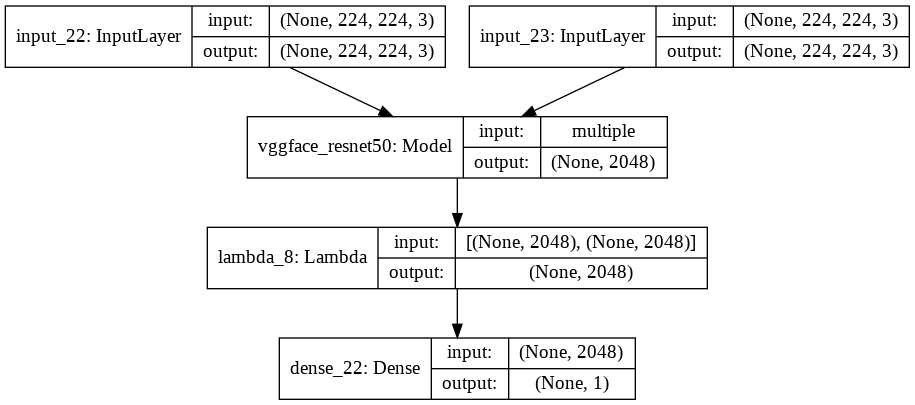
\includegraphics[scale=0.4]{img/base-resnet50.png}
    \caption{Arquitectura de la red siamesa utilizando \texttt{ResNet-50}.}
    \label{fig:base-resnet50}
\end{figure}


\begin{figure}[H]
    \centering
    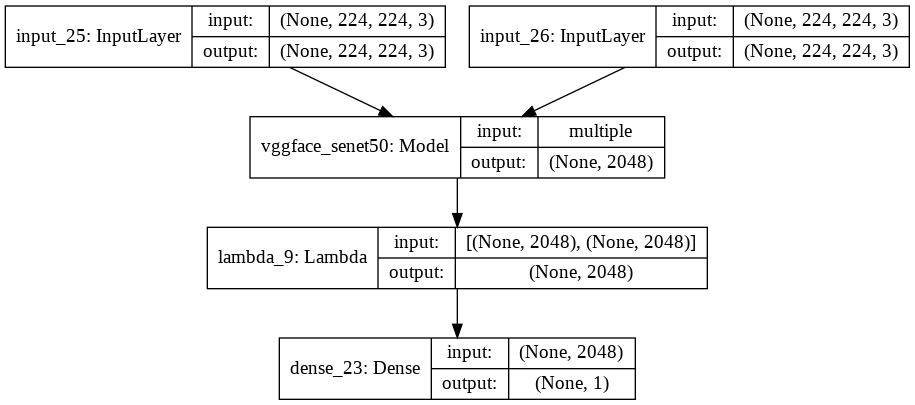
\includegraphics[scale=0.4]{img/base-senet50.png}
    \caption{Arquitectura de la red siamesa utilizando \texttt{SeNet-50}.}
    \label{fig:base-senet50}
\end{figure}


\begin{figure}[H]
    \centering
    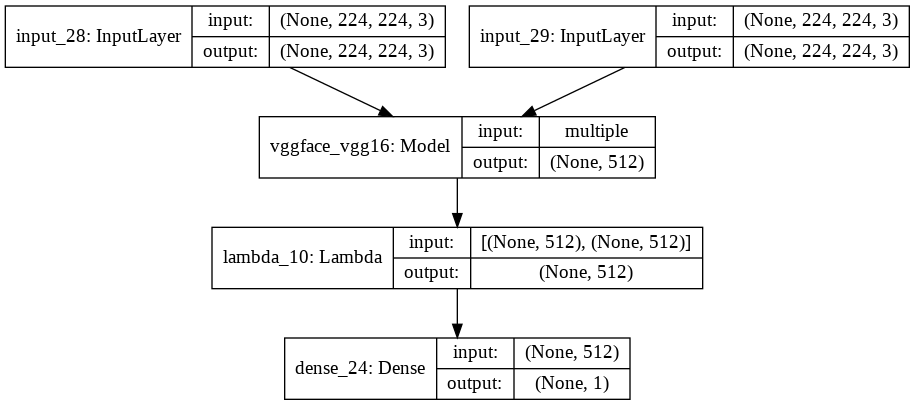
\includegraphics[scale=0.4]{img/base-vgg16.png}
    \caption{Arquitectura de la red siamesa utilizando \texttt{VGG16}.}
    \label{fig:base-vgg16}
\end{figure}

Estas serán las arquitecturas base que compararemos para determinar cuál de ellas es la más adecuada
para introducir mejoras.

\subsection{Método y parámetros de entrenamiento}

Vamos a hablar brevemente sobre cómo hemos entrenado las redes y qué parámetros hemos utilizado para
ello, justificando las decisiones que hemos tomado.

Hace falta decir, antes de continuar, que todas las pruebas se han realizado en un entorno de Colab
con GPU ya que las gráficas de las que disponemos no tienen tanta potencia como la que ofrece el entorno
de Google.

Lo primero que hace falta destacar es que vamos a entrenar todas las capas de la red, haciendo por tanto
\textit{fine-tuning} de la red. De esta forma, aprovecharemos el conocimiento que ya tienen
las redes preentrenadas y lo adaptaremos al problema en cuestión.

Entrenaremos cada modelo durante un total de 30 épocas, dando 100 pasos por época para entrenar y 30 para validar.
Como solo vamos a hacer \textit{fine-tuning} de la red, utilizar un número de épocas superior no se ha visto
necesario, ya que solo nos interesa ajustar ligeramente la red al problema. Si quisiéramos entrenar toda la red
de 0, tendríamos que poner muchísimas más épocas. Además de esto, 30 épocas nos ha permitido obtener, en general,
unos resultados no del todo malos, tal y como veremos maś adelante. En cuanto al número de pasos, se ha considerado
que 100 pasos de entrenamiento es suficiente, ya que los \textit{batches} que se generen en cada épocas serán, en
general, muy diferentes a los que se han generado anteriormente. En cuando a los 30 de validación, se ha considerado
suficiente, ya que estamos haciendo casi un tercio de los pasos de entrenamiento para validar.

En cuanto al tamaño del \textit{batch}, nuestra idea inicial era utilizar un \textit{batch} de tamaño 64, ya
que es un buen tamaño para entrenar redes grandes y en general permite obtener unos buenos resultados. Sin
embargo, esta idea se ha visto truncada rápidamente al ver que incluso la GPU de la que disponemos en el
entorno no puede asignar suficiente memoria a tensores que utilicen un \textit{batch} de dicho tamaño. Por tanto,
nos hemos visto obligados a disminuir el tamaño del \textit{batch} a 32. Además, con un tamaño de \textit{batch}
de 32 también podemos conseguir buena generalización, ya que podemos converger a un \textit{flat minimizer} \cite{DBLP:journals/corr/KeskarMNST16} igual que con uno de tamaño 64.

Otra cosa muy importante que hace falta establecer es la proporción de parientes que formarán los \textit{batches}
de entrenamiento y de validación. Para determinar el valor, hemos ido haciendo pruebas con distintos valores. En
general, parece que tener al menos un 50\% de casos positivos en los \textit{batches} de entrenamiento permite
ofrecer unos resultados aceptables. Si es menor a este valor, se ha visto que las redes no aprenden lo suficiente,
es decir, tendremos una mayoría de individuos no relacionados entre sí (casos sencillos de clasificar) y una minoría
de individuos con parentesco (casos más difíciles para nuestra red). Después de las pruebas llevadas a cabo, hemos
decidido que el 60\% del \textit{batch} (una proporción de 0.6) de entrenamiento y de validación serán ejemplos
positivos, ya que en un problema como el nuestro es más conveniente aumentar la cantidad de datos complicados a
la hora de entrenar. Tampoco podremos subir mucho este valor, ya que si descuidamos los individuos sin parentesco,
corremos el riesgo de que no aprenda nada de éstos y causar \textit{overfit}. Obviamente, dar con el valor óptimo
es muy complicado, por tanto nos podemos conformar con este valor.

En cuanto al optimizador utilizado, hemos probado \texttt{Adam} con los parámetros por defecto,
ya que es, por convenio, uno de los más utilizados, es eficiente y suele obtener unos buenos resultados.

Por último, utilizaremos inicialmente como función de pérdida la \textit{binary crossentropy} porque estamos en un
problema binario (dadas dos imágenes, determinar si son parientes o no). Por tanto, para problemas de este tipo
se suele utilizar esta función de pérdida.

\subsection{Método de comparación}

Para comparar los modelos, vamos a observar por una parte las gráficas de pérdida o \textit{loss} y de
\textit{accuracy} en los conjuntos de entrenamiento y validación, y por otra observaremos la \textit{accuracy}
que hayamos conseguido en \textit{Kaggle} al probar el modelo con los datos de test. En cuanto a la \textit{accuracy},
nos fiaremos algo más de la que nos proporciona \textit{Kaggle}, ya que desconocemos el valor umbral a partir
del que dos personas se pueden considerar pariente. Por tanto, es posible que los resultados obtenidos por
\texttt{Keras} tiren a la baja o a la alta. Es importante destacar que en \textit{Kaggle} se calculan dos
\textit{accuracies}: una privada con la mitad de los resultados, y una pública con la otra mitad. Por tanto,
los valores obtenidos pueden variar algo cada vez que subimos el mismo fichero, aunque van a ser parecidos.
Nosotros nos fijaremos en la \textit{accuracy} pública, ya que creemos que es la manera más justa de comparar
los modelos.

Para tomar la decisión final consideraremos las dos cosas anteriormente mencionadas. Además, meditaremos sobre
si existen diferencias significativas entre los resultados obtenidos.
\subsection{Resultados de la experimentación}

Vamos a analizar ahora los resultados obtenidos al entrenar las redes con las condiciones anteriormente
descritas. Vamos primero con los resultados para \texttt{ResNet-50}:

\begin{figure}[H]
\centering
\begin{minipage}{0.5\textwidth}
  \centering
  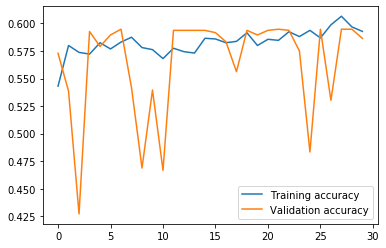
\includegraphics[scale=0.5]{img/accuracy-resnet50.png}
\end{minipage}%
\begin{minipage}{0.5\textwidth}
  \centering
  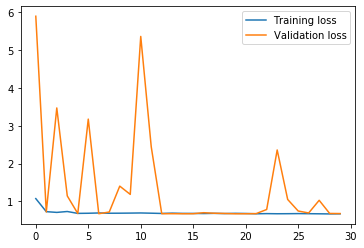
\includegraphics[scale=0.5]{img/loss-resnet50.png}
\end{minipage}
\caption{Evolución en el entrenamiento de \texttt{ResNet-50}.}
\label{fig:graph-resnet50}
\end{figure}

\begin{figure}[H]
    \centering
    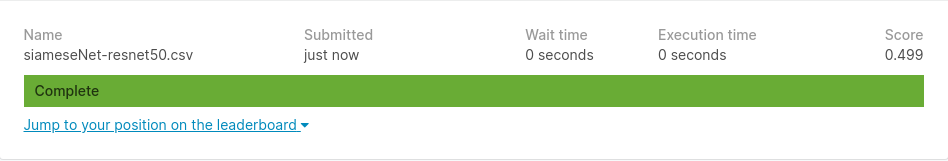
\includegraphics[scale=0.55]{img/siameseNet-resnet50.png}
    \caption{Resultados en el test de \texttt{ResNet-50}.}
    \label{fig:test-resnet50}
\end{figure}

Si observamos las gráficas de la figura \ref{fig:graph-resnet50}, vemos que la \textit{loss} en entrenamiento
es bastante baja y la \textit{accuracy} se queda en torno a 0.6 en las últimas épocas. No obstante, la
pérdida en validación oscila mucho, ya que hay algunas épocas en las que está pegada a la de entrenamiento,
mientras que en otras está muy por encima. Con la \textit{accuracy} pasa algo similar, ya que hay casos en los
que se queda muy por debajo de la de entrenamiento, otros donde queda por encima y otros donde más o menos son
iguales. Estas oscilaciones pueden deberse a que, debido a la forma en la que se generan los datos de validación,
puede que en alguna época haya casos más difíciles y en otras más fáciles, ya que al escoger de forma aleatoria
no tenemos control sobre cuántos casos fáciles y difíciles se meten; solo controlamos los positivos y los negativos.

Los resultados obtenidos en \textit{Kaggle}, los cuáles se pueden ver en la figura \ref{fig:test-resnet50},
muestran que la red tiene una \textit{accuracy} en torno a 0.5. Este valor es bastante bajo, ya que perfectamente
podríamos utilizar un modelo más simple que siempre devuelva 0 o siempre devuelva 1, de forma que se acierte más
o menos la mitad de los casos.

Los resultados para \texttt{SeNet-50} son los siguientes:

\begin{figure}[H]
\centering
\begin{minipage}{0.5\textwidth}
  \centering
  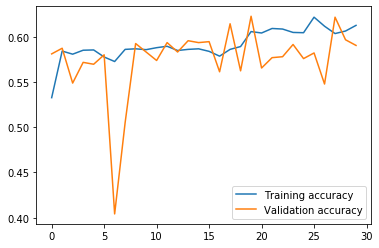
\includegraphics[scale=0.5]{img/accuracy-senet50.png}
\end{minipage}%
\begin{minipage}{0.5\textwidth}
  \centering
  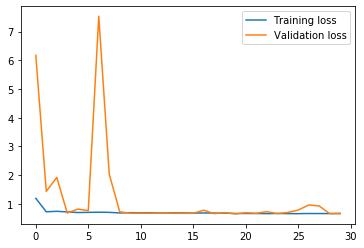
\includegraphics[scale=0.5]{img/loss-senet50.png}
\end{minipage}
\caption{Evolución en el entrenamiento de \texttt{SeNet-50}.}
\label{fig:graph-senet50}
\end{figure}

\begin{figure}[H]
    \centering
    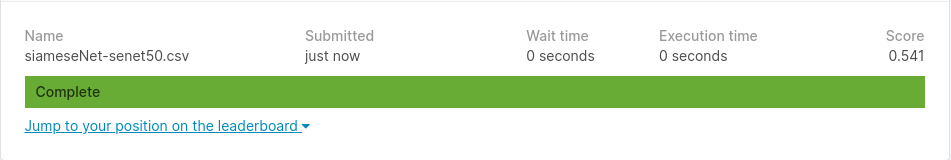
\includegraphics[scale=0.55]{img/siameseNet-senet50.png}
    \caption{Resultados en el test de \texttt{SeNet-50}.}
    \label{fig:test-senet50}
\end{figure}

Si observamos la figura \ref{fig:graph-senet50}, vemos que los resultados son bastante parecidos a los que
habíamos obtenido para \texttt{ResNet-50} en la figura \ref{fig:graph-resnet50}. Vemos de nuevo que la pérdida
en validación se queda muy cerca de la de entrenamiento, pero siguen habiendo algunos picos. La \textit{accuracy}
en validación es muy parecida a la que teníamos anteriormente, aunque los picos son menos pronunciados que antes.

Ahora bien, si observamos los resultados de la figura \ref{fig:test-senet50}, vemos que la \textit{accuracy}
ha subido hasta aproximadamente 0.54. Por tanto, ha habido cierta mejora en ese aspecto. Es importante
destacar que la puntuación obtenida en \textit{Kaggle} puede variar algo cada vez que se suben los ficheros
de resultados, ya que se utiliza aproximadamente el 50\% de los resultados para obtener la puntuación. Aun así,
este modelo no lo ha hecho tan mal, aunque sigue estando demasiado cerca de ser un modelo que diga que clasifique
todas las parejas como positivas o como negativas.

Finalmente, veamos los resultados de \texttt{VGG16}:

\begin{figure}[H]
\centering
\begin{minipage}{0.5\textwidth}
  \centering
  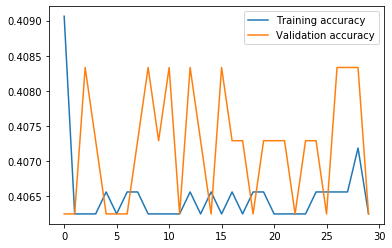
\includegraphics[scale=0.5]{img/accuracy-vgg16.png}
\end{minipage}%
\begin{minipage}{0.5\textwidth}
  \centering
  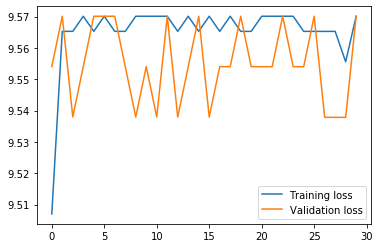
\includegraphics[scale=0.5]{img/loss-vgg16.png}
\end{minipage}
\caption{Evolución en el entrenamiento de \texttt{VGG16}.}
\label{fig:graph-vgg16}
\end{figure}

\begin{figure}[H]
    \centering
    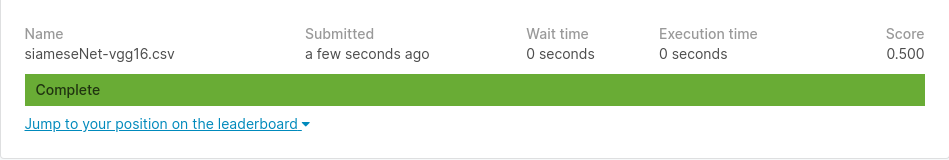
\includegraphics[scale=0.55]{img/siameseNet-vgg16.png}
    \caption{Resultados en el test de \texttt{VGG16}.}
    \label{fig:test-vgg16}
\end{figure}

Si observamos los gráficos de la figura \ref{fig:graph-vgg16}, vemos que sucede todo lo contrario
a lo que hemos visto hasta ahora. Vemos que la pérdida en entrenamiento crece en vez de disminuir a medida
que van pasando las épocas. Solo en las últimas empieza a bajar algo, aunque luego vuelve a subir. La pérdida
de validación oscila bastante, quedándose cerca de la de entrenamiento, aunque no parece tener un patrón claro y
tampoco parece mejorar. En cuanto a la \textit{accuracy}, vemos que esta baja en vez de subir en el conjunto de
entrenamiento, y sigue un comportamiento parecido al de la pérdida. La \textit{accuracy} de validación no parece
mejorar, ya que de nuevo parece oscilar en torno a la de entrenamiento. A pesar de que los resultados no van mejorando
a medida que pasan las épocas, vemos que en general están bastante cerca unos de otros. Por tanto, de aquí podemos
concluir que el modelo no aprende mucho y que se queda demasiado corto en comparación a los anteriores, ya que los
resultados son mucho peores que los anteriores, ya que la pérdida al final se queda en torno al 9.57 y la
\textit{accuracy} en torno a 0.4, teniendo en cuenta que en los modelos anteriores la pérdida bajaba
de 1 y la \textit{accuracy} llegaba hasta aproximadamente 0.6.

Ahora bien, si observamos los resultados de la figura \ref{fig:test-vgg16}, vemos que obtiene una puntuación de
0.5, casi igual que la de \texttt{ResNet-50}. A simple vista, podríamos decir que ambos modelos funcionan más
o menos de manera similar, aunque tras observar las gráficas de la figura \ref{fig:graph-vgg16} podemos ver
que no es así.

\subsection{Elección del mejor modelo base}

Una vez que hemos visto los resultados obtenidos por cada modelo, vamos a escoger el mejor de ellos. Ya desde
el principio, \texttt{VGG16} está descartado, ya que es un modelo que se queda demasiado corto. Ahora, la decisión
está entre \texttt{ResNet-50} y \texttt{SeNet-50}.

En un principio nos decantamos por \texttt{SeNet-50} por los pequeños detalles vistos anteriormente, como puede ser la
precisión obtenida en el conjunto de test o los gráficos con picos menos abruptos. No obstante, al realizar varias
pruebas con ella, vimos que la respuesta a las mejoras que nos estaba dando no estaba siendo tan buena como la que nos
daba \texttt{ResNet-50}, así que decidimos seguir experimentando con este último modelo.

Una de las razones por las que no ha funcionado ha podido ser la propia arquitectura de la red. \texttt{SeNet-50}
utiliza varias redes existentes como la propia \texttt{ResNet-50}, pero añadiéndole un bloque \texttt{SE}
(\textit{Squeeze and Excitation}), el cual tiene la siguiente estructura:

\begin{figure}[H]
    \centering
    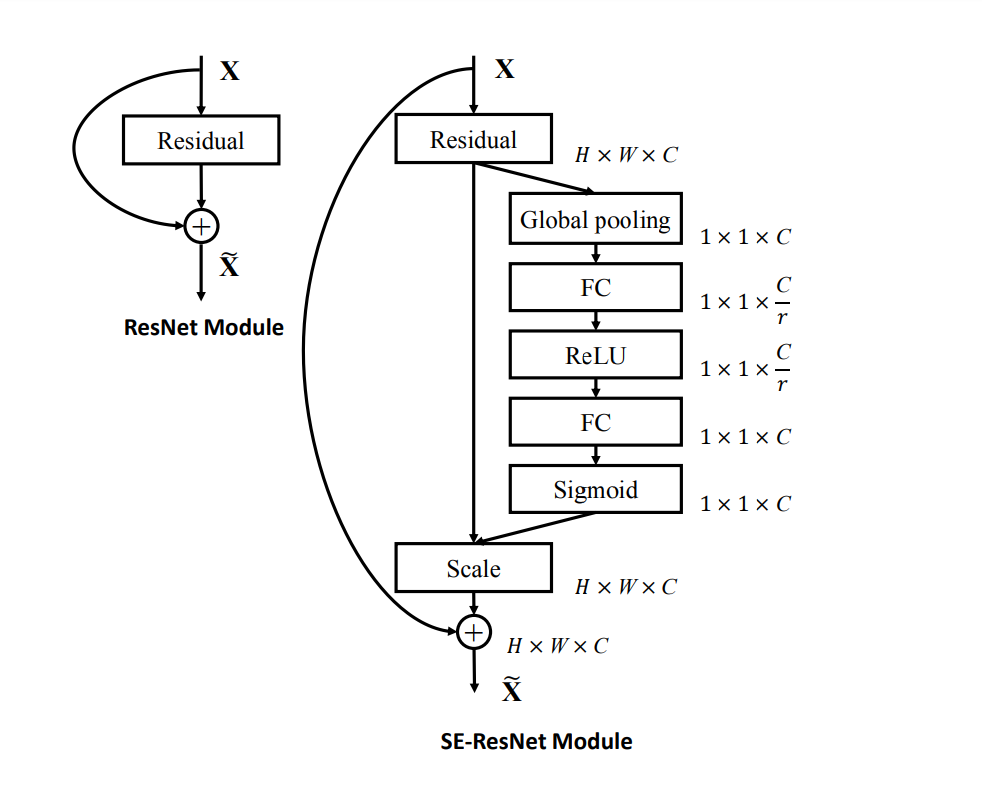
\includegraphics[scale=0.45]{img/senet-arch.png}
    \caption{Arquitectura del módulo residual original (izquierda) y del módulo \texttt{SeNet-50} (derecha).
    \protect\cite{DBLP:journals/corr/abs-1709-01507}}
    \label{fig:senet-arch}
\end{figure}

Como podemos observar, este bloque utiliza varias capas \textit{Fully-Connected} y de activación tras las capas
residuales, con el objetivo de destacar las características verdaderamente importantes y suprimir las menos útiles.
Sin embargo, con las mejoras implementadas en la siguiente sección, veremos cómo podemos compensar la ausencia de ese
bloque y obtener unos resultados bastante buenos con \texttt{ResNet-50}, siendo incluso mejores que los obtenidos
al aplicar las mejoras sobre \texttt{SeNet-50}. Aparte de eso, también conseguimos cierto ahorro de cómputo, ya que
entrenar \texttt{ResNet-50} es más rápido que entrenar a \texttt{SeNet-50}.


\section{\textsc{Mejora de la red base}}

Una vez que hemos elegido el modelo base que queremos mejorar, vamos a probar a realizar algunas modificaciones
a la arquitectura de la red, al optimizador utilizado, a la función de pérdida, etc.

\subsection{Reducción del \textit{Learning Rate} de \texttt{Adam}}

La primera modificación que vamos a proponer va a ser la modificación del optimizador. Decidimos utilizar \texttt{Adam}
ya que es uno de los más utilizados por sus buenos resultados, pero lo implementamos con los parámetros por defecto, es
decir, con un $learning\_rate=0.001$. Como hemos podido comprobar en las ejecuciones iniciales, las gráficas llegaban a
su valores más altos muy pronto, lo que que quiere decir que estamos aprendiendo un conjunto de pesos por debajo del
óptimo demasiado rápido y provocando además un entrenamiento muy inestable.

En consecuencia, vamos a bajar el valor de este parámetro a $learning\_rate=0.00001$, que en un principio puede resultar
bastante pequeño, pero viendo como han salido los primeros resultados, pensamos que funcionará correctamente. Estos han
sido los resultados obtenidos:

\begin{figure}[H]
\centering
\begin{minipage}{0.5\textwidth}
  \centering
  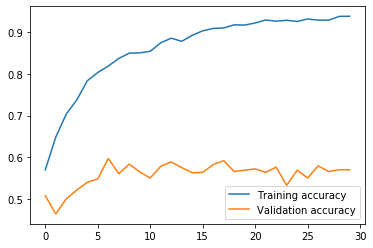
\includegraphics[scale=0.5]{img/accuracy-adam.png}
\end{minipage}%
\begin{minipage}{0.5\textwidth}
  \centering
  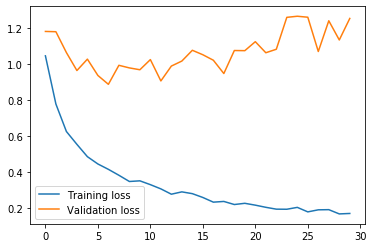
\includegraphics[scale=0.5]{img/loss-adam.png}
\end{minipage}
\caption{Evolución en el entrenamiento de \texttt{Adam} con reducción del LR.}
\label{fig:graph-adam}
\end{figure}

\begin{figure}[H]
    \centering
    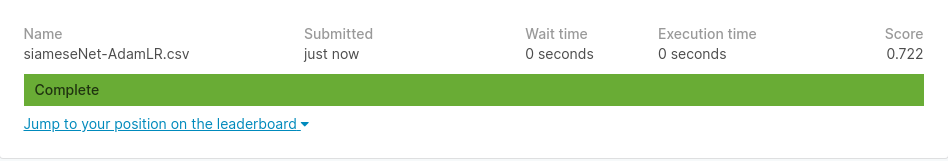
\includegraphics[scale=0.55]{img/siameseNet-AdamLR.png}
    \caption{Resultados en el test de \texttt{Adam} con reducción del LR.}
    \label{fig:test-adam}
\end{figure}

Como podemos comprobar, las gráficas \ref{fig:graph-adam} son completamente diferentes a las anteriores. Vemos como en
esta ocasión, la curva del \textit{accuracy} en el entrenamiento sí va aumentando paulatinamente y de una forma mucho
mas suave (podemos observar no hay tantos picos ni irregularidades como antes). Lo mismo sucede con la curva de pérdida
en el entrenamiento, aunque en este caso, en vez de aumentar, decrece. En cuanto a los resultados obtenidos en validación,
pese a que no hemos conseguido mejorar tanto los resultados, sí hemos obtenido unas líneas un poco más regulares y sin
valores tan extremos como en las ejecuciones iniciales, donde alcanzábamos picos de hasta 0.42 en \textit{accuracy} o de
5.5 en la función de pérdida, aproximadamente.

Si observamos los resultados del test en la figura \ref{fig:test-adam}, podemos observar como el cambio ha sido considerable.
Hemos pasado de tener una precisión del 50\% a tener una del 72.2\%. Esto quiere decir que hemos hecho bastante
bien reduciendo este valor, ya que hemos podido comprobar que estaba aprendiendo demasiado rápido con unos pesos que no eran
los más óptimos. Gracias a esto, podemos decir que la elección de un buen optimizador y sus parámetros es muy importante,
porque de llegar a pensar que nuestro modelo es peor que un clasificador que ponga todas las parejas positivas o negativas,
hemos pasado a tener un modelo bastante prometedor.


\subsection{Inserción de capas densas}

A la vista de los resultados que hemos obtenido con la mejora anterior, vamos a probar a añadirle algunas capas densas
más al final para ver cómo se comporta el modelo (conservando claro está la mejora anterior).

Vamos a introducir dos capas densas antes de la neurona de salida, y entre ellas vamos a meter capas de \textit{dropout}
con una probabilidad pequeña (0.1 por ejemplo), de forma que se regularice ligeramente el modelo y se evite el
\textit{overfit}. De esta forma, podemos hacer más operaciones con la distancia que hemos calculado, obteniendo
posiblemente mejores resultados al tener algunas capas más. Nos hemos inspirado en uno de los proyectos de \textit{Kaggle}
\cite{best-project}, ya que utilizaba esta combinación de capas y obtenía buenos resultados (no utilizamos nada
más de la arquitectura, ya que es completamente diferente a lo que nosotros hemos hecho).

Para insertar dichas capas, solo tenemos que modificar la función que se puede ver en el listado \ref{lst:base-net},
de forma que se incluyan las capas \texttt{Dense} de la siguiente forma:

\begin{lstlisting}
# Aniadimos la funcion de distancia
L1_distance = L1_layer([encoded_l, encoded_r])

# Aniadimos 2 capas FC y otras 2 de Dropout tras cada una
x = Dense(100, activation="relu")(L1_distance)
x = Dropout(0.1)(x)
x = Dense(25, activation="relu")(x)
x = Dropout(0.1)(x)

# Aniadimos la ultima capa sigmoidal a la red
prediction = Dense(1, activation='sigmoid')(x)
\end{lstlisting}

La arquitectura del modelo, una vez que se ha compilado, es la siguiente:

\begin{figure}[H]
    \centering
    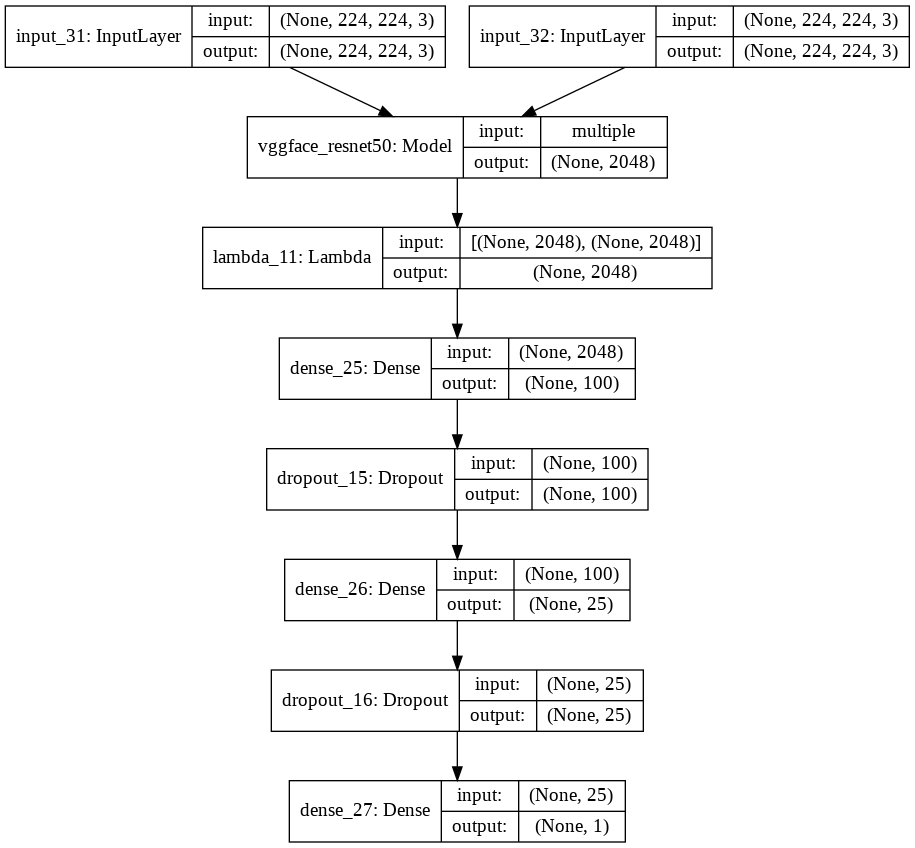
\includegraphics[scale=0.4]{img/base-dense.png}
    \caption{Arquitectura de nuestro modelo añadiendo capas FC.}
    \label{fig:base-dense}
\end{figure}

Tras entrenar la red, obtuvimos los siguientes resultados:

\begin{figure}[H]
\centering
\begin{minipage}{0.5\textwidth}
  \centering
  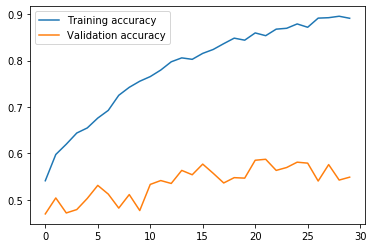
\includegraphics[scale=0.5]{img/accuracy-dense.png}
\end{minipage}%
\begin{minipage}{0.5\textwidth}
  \centering
  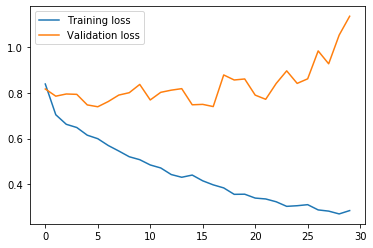
\includegraphics[scale=0.5]{img/loss-dense.png}
\end{minipage}
\caption{Evolución en el entrenamiento añadiendo capas FC.}
\label{fig:graph-dense}
\end{figure}

\begin{figure}[H]
    \centering
    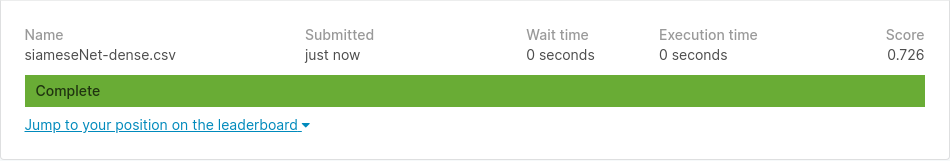
\includegraphics[scale=0.55]{img/siameseNet-dense.png}
    \caption{Resultados en el test añadiendo capas FC.}
    \label{fig:test-dense}
\end{figure}

Si observamos la figura \ref{fig:graph-dense}, vemos que, en general, los resultados obtenidos son parecidos a los que
teníamos antes, si bien es cierto que hay pequeñas diferencias. Por una parte, la \textit{accuracy} en el conjunto de
entrenamiento sube de manera algo más lenta, y se queda parada un poco por debajo de la que se puede ver
en la figura \ref{fig:graph-adam}. La pérdida del conjunto de entrenamiento también se queda algo por encima
a la que teníamos antes. En cuanto a los resultados en el conjunto de validación, vemos que la \textit{accuracy}
es más o menos igual a la que teníamos anteriormente, mientras que la pérdida es algo más baja, aunque comienza a subir
en las últimas épocas, lo cuál es un posible síntoma de \textit{overfit}. No obstante, los resultados no son para
nada malos si los comparamos con los que teníamos en un principio, ya que aquí los resultados de validación están,
de nuevo, más estabilizados que los de antes.

Los resultados son completamente lógicos teniendo en cuenta que hemos introducido más capas. Al tener más capas,
la convergencia es algo más lenta, ya que hay más parámetros que optimizar. Por tanto, es normal que los resultados
estén algo por debajo de lo que teníamos con un modelo más simple.

Ahora, si observamos la \textit{accuracy} obtenida con el conjunto de test, el cuál puede ser visto en la figura
\ref{fig:test-dense}, vemos que ha habido una mejora casi despreciable respecto a la \textit{accuracy} obtenida
anteriormente (solo 4 milésimas). Por tanto, la mejora ha permitido mejorar los resultados pero en una
cantidad muy, muy pequeña. A pesar de eso, vamos a conservarla, ya que hay ciertas cosas que podemos probar sobre
esta modificación que nos pueden permitir obtener unos mejores resultados, tal y como veremos más adelante.

\subsection{Cambio del optimizador: \texttt{RMSProp}}

Ya que hasta ahora hemos venido utilizando el optimizador \texttt{Adam}, hemos querido probar con otro para
ver si se produce alguna mejora o no. Vamos a probar el optimizador \texttt{RMSProp} sobre la red de la sección
anterior. \texttt{RMSProp} es un optimizador con \textit{learning rate} adaptativo el cuál es bastante conocido y
utilizado, ya que permite obtener unos buenos resultados y es rápido. En este caso, vamos a utilizar el optimizador
con los parámetros por defecto, lo cuál viene a significar que utilizaremos un \textit{learning rate} de 0.001.

Los resultados que hemos obtenido al entrenar el modelo se pueden ver a continuación:

\begin{figure}[H]
\centering
\begin{minipage}{0.5\textwidth}
  \centering
  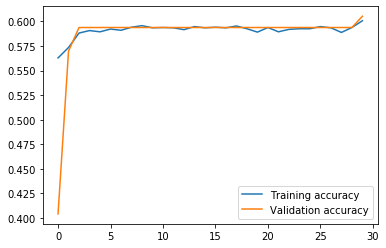
\includegraphics[scale=0.5]{img/accuracy-rmsprop.png}
\end{minipage}%
\begin{minipage}{0.5\textwidth}
  \centering
  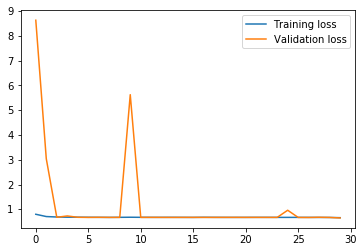
\includegraphics[scale=0.5]{img/loss-rmsprop.png}
\end{minipage}
\caption{Evolución en el entrenamiento con el optimizador RMSProp.}
\label{fig:graph-rmsprop}
\end{figure}

\begin{figure}[H]
    \centering
    \includegraphics[scale=0.55]{img/siameseNet-rmsprop.png}
    \caption{Resultados en el test con el optimizador RMSProp.}
    \label{fig:test-rmsprop}
\end{figure}

Si observamos las gráficas de la figura \ref{fig:graph-rmsprop}, vemos un claro ejemplo de estancamiento. Vemos
que la \textit{accuracy} en entrenamiento no mejora mucho a pesar de que van pasando las épocas. Lo mismo sucede
para la función de pérdida, ya que se mantiene casi constante durante todo el entrenamiento. En cuanto al conjunto
de validación, vemos que la curva de pérdida se pega bastante a la del conjunto de entrenamiento, a pesar de que
hay ciertos picos. Lo mismo sucede para la curva del \textit{accuracy}, ya que se pega bastante bien a la de
entrenamiento. No obstante, aunque los resultados no parezcan del todo malos a primera vista, se quedan en general
bastante cortos con los que hemos visto anteriormente, donde teníamos mucha más \textit{accuracy} y una pérdida
más pequeña.

Este descenso en los resultados durante el entrenamiento va a afectar a los obtenidos en el conjunto de test.
Tal y como podemos ver en la figura \ref{fig:test-rmsprop}, la \textit{accuracy} obtenida es tan solo 0.591.
Esto representa un retroceso muy importante respecto a lo que teníamos anteriormente. Por tanto, en este caso no nos
ha merecido la pena probar este optimizador con esta configuración de parámetros concreta, ya que el modelo
se queda estancado demasiado rápido y no permite obtener unos buenos resultados.

\subsection{Cambio de la función de pérdida: \textit{Focal Loss}}

Al igual que hemos decidido cambiar el optimizador, vamos a cambiar también la función de pérdida. La función que
se suele utilizar es la \textit{binary\_crossentropy}, que es la que nosotros hemos seleccionado por defecto. Pese a
esto, queremos probar otra función a ver que tal funciona en nuestro modelo.

Hemos decidido utilizar la función \textit{Focal Loss} de forma que se disminuya la pérdida de ejemplos bien clasificados,
algo bastante importante en el problema que estamos abordando. Lo que hace la función es centrarse en los ejemplos
difíciles, de forma que los ejemplos que sean más fáciles de clasificar aporten menos a la función de pérdida que
aquellos que sean más difíciles. Para evaluar la efectividad del modelo se puede revisar el artículo original
\cite{DBLP:journals/corr/abs-1708-02002}.

A la hora de implementar esta función de pérdida hemos utilizado un modelo del siguiente repositorio \cite{focal-loss}.
La ejecución se ha realizado con el código acumulativo hasta la segunda mejora (donde se implementaban las capas densas)
ya que el cambio de optimizador no funcionó todo lo bien que se esperaba. Los resultados han sido los siguientes:

\begin{figure}[H]
\centering
\begin{minipage}{0.5\textwidth}
  \centering
  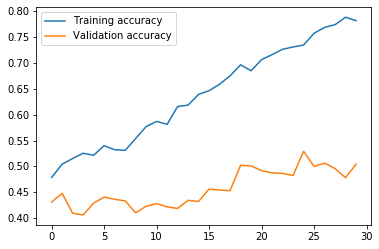
\includegraphics[scale=0.5]{img/accuracy-focalloss.png}
\end{minipage}%
\begin{minipage}{0.5\textwidth}
  \centering
  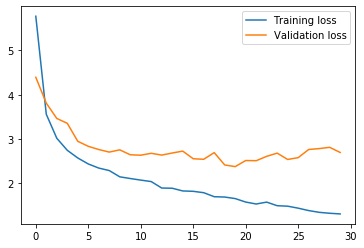
\includegraphics[scale=0.5]{img/loss-focalloss.png}
\end{minipage}
\caption{Evolución en el entrenamiento con la función de pérdida Focal Loss.}
\label{fig:graph-focalloss}
\end{figure}

\begin{figure}[H]
    \centering
    \includegraphics[scale=0.55]{img/siameseNet-focalloss.png}
    \caption{Resultados en el test con la función de pérdida Focal Loss.}
    \label{fig:test-focalloss}
\end{figure}

Como podemos observar en la figura \ref{fig:graph-focalloss}, la progresión del \textit{accuracy} en entrenamiento y
en validación ha ido según lo esperando, ya que son líneas bastante suaves y sin muchas irregularidades.
Aunque por otro lado, los valores máximos a los que han llegado no han sido tan altos como antes. Esto puede deberse
a que el número de épocas quizás era demasiado bajo y tendríamos que haberle dejado más tiempo para entrenar, o también
a que la tasa de aprendizaje de nuestro optimizador es muy baja para esta nueva función de pérdida. También podemos
ver que en el gráfico con la función de pérdida, pese a que empiezan en valores muy altos, las funciones van
decreciendo de una forma bastante suave hasta obtener valores bastante aceptables. Esto quiere decir que la función
ha realizado su trabajo como esperábamos reduciendo la pérdida de los ejemplos bien clasificados.

Si observamos la figura \ref{fig:test-focalloss}, el resultado obtenido no ha sido malo, pero no tan bueno como nos
esperábamos en un principio. La puntuación obtenida está sólo un 2\% por debajo de la mejor obtenida hasta ahora.
No obstante, como esta función de pérdida está diseñada para problemas como el nuestro, se esperaba que fuese a ir
mejor. En nuestro caso, nos quedaremos con la función de \textit{binary\_crossentropy} para las siguientes mejoras,
pero una buena propuesta de mejora del modelo sería el estudio en mayor profundidad de la \textit{Focal Loss} (ya sea
aumentando las épocas como hemos dicho antes, el \textit{learning rate} del optimizador o cambiando algún parámetro
interno de la propia función).

\subsection{Inicialización y regularización de las capas densas}

La siguiente mejora propuesta es la inicialización de los pesos y del \textit{bias}, y la regularización del kernel.
Para las inicializaciones utilizaremos una distribución normal de media 0 y desviación típica 0.01 en cuanto a los
pesos; y con media 0.5 y desviación típica 0.01 para el \textit{bias}. La función que utilizaremos la hemos obtenido
del siguiente repositorio \cite{initializers}. En cuanto a la regularización del kernel, vamos a utilizar la 
regularización L2. El motivo por el que utilizamos estos valores se debe al siguiente artículo \cite{msc-thesis}, en
el cual recomienda estas inicializaciones y la regularización L2 para las CNN.

En nuestra red siamesa, simplemente tendremos que modificar las capas densas añadiéndole como parámetros los valores
mencionados. La implementación de nuestro código es la siguiente:

\begin{lstlisting}
    # Aniadimos 2 capas FC inicializadas y regularizadas,
    # y otras 2 de Dropout tras cada una
    x = Dense(100, activation="relu", 
                        kernel_regularizer=regularizers.l2(1e-3),
                        kernel_initializer=initialize_weights,
                        bias_initializer=initialize_bias)(L1_distance)
    x = Dropout(0.1)(x)
    x = Dense(25, activation="relu",
                        kernel_regularizer=regularizers.l2(1e-3),
                        kernel_initializer=initialize_weights,
                        bias_initializer=initialize_bias)(x)
    x = Dropout(0.1)(x)

    # Aniadimos la ultima capa sigmoidal a la red
    prediction = Dense(1, activation='sigmoid',
                        bias_initializer=initialize_bias)(x)
\end{lstlisting}

Este ha sido el resultado de entrenar el modelo:

\begin{figure}[H]
\centering
\begin{minipage}{0.5\textwidth}
  \centering
  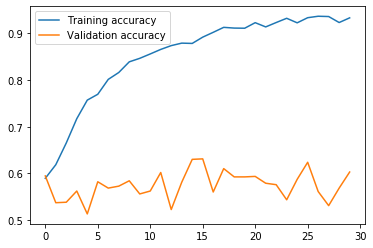
\includegraphics[scale=0.5]{img/accuracy-regularizers.png}
\end{minipage}%
\begin{minipage}{0.5\textwidth}
  \centering
  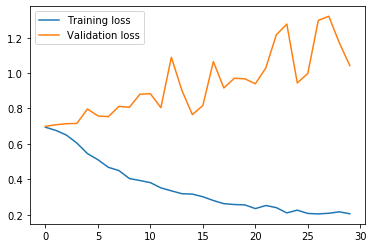
\includegraphics[scale=0.5]{img/loss-regularizers.png}
\end{minipage}
\caption{Evolución en el entrenamiento con las capas FC regularizadas e inicializadas.}
\label{fig:graph-regularizers}
\end{figure}

\begin{figure}[H]
    \centering
    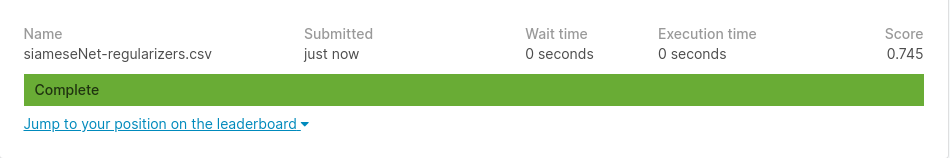
\includegraphics[scale=0.55]{img/siameseNet-regularizers.png}
    \caption{Resultados en el test con las capas FC regularizadas e inicializadas.}
    \label{fig:test-regularizers}
\end{figure}

Los resultados mostrado en la figura \ref{fig:graph-regularizers} también son bastante similares a los que obtuvimos
con las mejoras que sí funcionaron, lo cual ya es indicativo de que esta ejecución no ha ido mal. Si analizamos cada uno
de los gráficos, podemos ver que la \textit{accuracy} a la hora de entrenar es ligeramente mejor que en el resto de
modelos, mientras que en validación sigue siendo una línea bastante irregular. En cuanto a las funciones de pérdida,
ha sucedido más de lo mismo, ya que la de entrenamiento ha sido la que ha obtenido los valores más bajos en comparación
al resto de modelos, pero la de validación incluso ha ido aumentando. Esto puede deberse a que estemos empezando a
sobreentrenar, aunque no lo tendremos muy en cuenta porque los valores siguen siendo muy bajos y los resultados finales
bastante buenos.

Estos resultados finales, como podemos ver en la figura \ref{fig:test-regularizers}, son los mejores que hemos obtenido
hasta ahora, llegando al 0.745 de precisión. Esto quiere decir que la inicialización y regularización en las
capas densas es una mejora a tener en cuenta. Nosotros sólo la hemos implementado en las últimas capas (añadidas por
nosotros mismos), pero en caso de no utilizar una red ya preentrenada o querer modificar la implementación de la que ya
tenemos, puede llegar a funcionar bastante bien.

\subsection{Resultados finales}

Por último, vamos a mostrar los resultados obtenidos de todas propuestas de mejora para nuestra red siamesa. Junto a ellos,
también mostraremos las puntuaciones privadas con la otra mitad del conjunto y las analizaremos:

\begin{figure}[H]
    \centering
    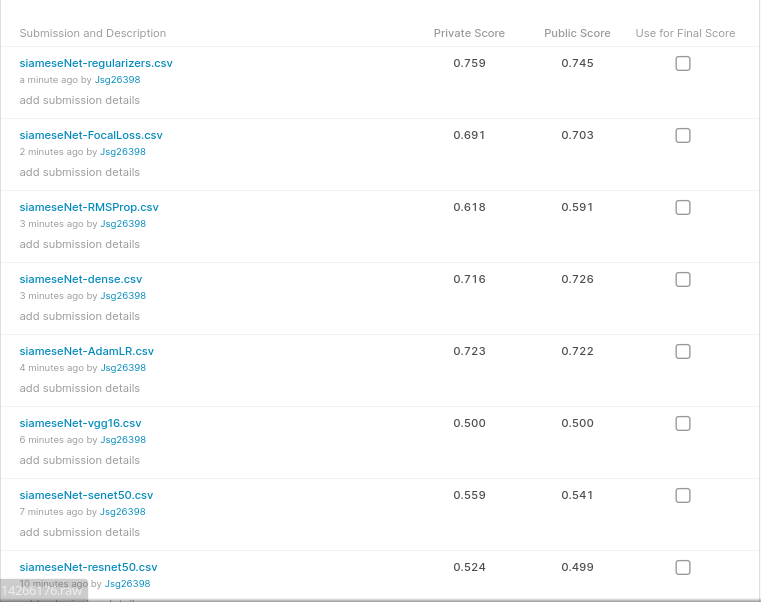
\includegraphics[scale=0.7]{img/siameseNet.png}
    \caption{Resultados de todos los test (private y public score).}
    \label{fig:test-regularizers}
\end{figure}

Como podemos observar, en general, no hay mucha diferencia entre los resultados públicos y los privados. Vemos que en la
mayoría de casos los resultados no se corresponden debido a que se utilizan datos distintos. Vemos también que el modelo
que obtiene mejores resultados en ambas puntuaciones es el modelo regularizado, quedando bastante por encima de los otros.
Vemos que el modelo base con \texttt{RESNET50} es el que obtiene peores resultados para los tests públicos, mientras
que el modelo base con \texttt{VGG16} es el que obtiene peores resultados para los privados. Gracias a esta imagen
podemos ver la evolución de nuestro modelo, como ha pasado de ser casi tan malo como un modelo que siempre devuelve
0 o 1 a un modelo que es capaz de discernir en cierto grado individuos que son parientes de los que no lo son.

\section{Conclusiones}

En este proyecto nos hemos enfrentado a un problema muy difícil, el cuál es determinar si dos individuos están
emparentados a partir de fotos de sus caras. Para abordar el problema, hemos procesado los datos y hemos montado
una serie de redes siamesas base a partir de redes preentrenadas con imágenes de caras. De entre estos modelos base,
hemos escogido el que creíamos que era el mejor. A este modelo escogido hemos probado a aplicarle una serie de
mejoras, hasta que hemos dado con una buena combinación que nos ha permitido obtener unos resultados bastante buenos.

A pesar de todo, sabemos que aun existe cierto margen de mejora. Se pueden intentar optimizar los parámetros de nuestra
red. Por ejemplo, podemos intentar ajustar mejor el \textit{learning rate} inicial, la \textit{Focal Loss} para ver si se
pueden conseguir mejores resultados aun, aplicar técnicas para detener el entrenamiento cuando la red se estanque, etc.
También podríamos intentar sacar alguna métrica más sofisticada que la distancia L1 entre los tensores de salida de las
dos redes que extraen características. Finalmente, se podría probar a crear un modelo sofisticado al hacer el ensamblado
de modelos más simples, aunque para hacer eso se necesitaría una máquina lo suficientemente potente.

En resumen, hemos probado nuestro enfoque con el problema y nos ha permitido obtener unos resultados bastante buenos,
aunque hay muchas más ideas que se podrían explorar para conseguir unos mejores resultados aun.

\newpage

\printbibliography

\end{document}
